Con il termine \emph{superficie estesa} ci si riferisce ad un solido soggetto a scambio termico per conduzione al proprio interno e per convezione attraverso il contorno. 
\begin{figure}
\centering
\psfrag{w}{$w$}
\psfrag{t}{$t$}
\psfrag{L}{$L$}
\psfrag{T0}{$T_0$}
\psfrag{hP}{$h_P$}
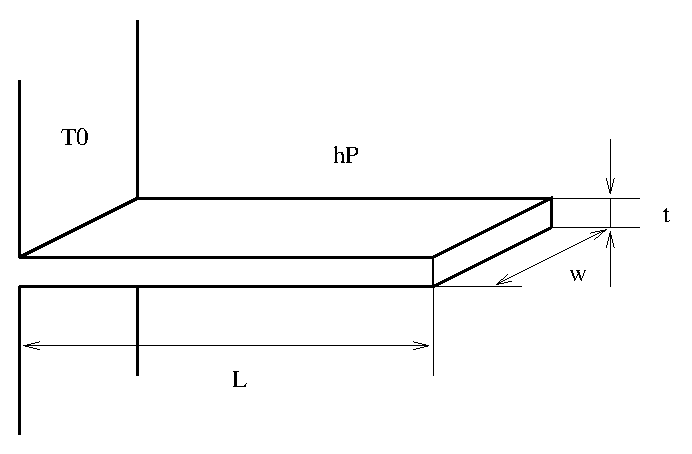
\includegraphics[width=0.5\textwidth]{./figures/eps/fin.eps}
\caption{Schema di un'aletta a base rettangolare e sezione costante.}
\label{fig:fin}
\end{figure}
Una superficie estesa utilizzata per migliorare lo scambio termico tra un solido ed il fluido che lo circonda \`e detta \emph{aletta} (si veda \figref{fig:fin}). Nel caso in cui il numero di Biot:
\begin{equation*}
\Biot \eqbydef \frac{h_P t w}{2 k \left( t + w \right)}
\end{equation*}
sia sufficientemente piccolo (tipicamente inferiore a $0.1$), si pu\`o assumere che la temperatura sia uniforme sulla sezione trasversale dell'aletta. Supponendo che la temperatura asintotica del fluido che lambisce l'aletta $T_{\infty}$ sia costante, il profilo di temperatura nella direzione longitudinale \`e fornito dall'equazione del calore monodimensionale:
\begin{equation}
-\frac{\ud^2 \theta}{\ud x^2} + a\theta = 0,\quad 0<x<L,
\label{eq:heat}
\end{equation}
ove si \`e posto $\theta\eqbydef T - T_{\infty}$ e $a \eqbydef 2h_P \left( w + t\right) / kwt$. Per fissare le condizioni al bordo, si assuma che la base dell'aletta sia alla temperatura della superficie $T_0$ e che non vi sia scambio di calore attraverso l'altra estremit\`a (condizione di \emph{punta adiabatica}):
\begin{equation*}
\function{\theta}{0} = T_0 - T_{\infty},\quad %
\function{\frac{\ud\theta}{\ud x}}{L} = 0.
\end{equation*}
Per maggiori dettagli si veda \cite{Incropera.DeWitt:1996}

Una soluzione approssimata dell'equazione precedente pu\`o essere ottenuta discretizzandola secondo il metodo delle differenze finite. Introduciamo una partizione uniforme $\Th$ dell'intervallo $\openint{0}{L}$ in $M$ elementi e consideriamo l'interpolante della soluzione ai nodi $x_j = jh$, $j=0,\ldots,M$, essendo $h\eqbydef L / M$ il passo di griglia. Indichiamo, inoltre, con $u_i=u_h(x_i)$, $i=0,\ldots,M$ i valori nodali della soluzione approssimata, che costituiscono le incognite del problema. Per le condizioni al bordo si ha che $u_0=\theta_0\eqbydef T_0 - T_{\infty}$. Si ottiene il seguente sistema lineare:
\begin{equation}
\label{eq:stfem}
A\mathbf{u}=\mathbf{b},
\end{equation}
essendo:
\begin{equation*}
\U=\left[u_0,\ldots,u_M\right]^T,\quad \mathbf{b}=\left[\theta_0,0,\ldots,0\right]^T,
\end{equation*}
e:
\begin{equation*}
\mathbb{R}^{(M+1)\times (M+1)}\ni A\eqbydef\left[
\begin{array}{ccccccc}
1       & 0         & 0         & \ldots    & 0         & 0     \\
-1      & 2+h^2 a   & -1        & \ldots    & 0         & 0     \\
\vdots  &           & \ddots    &           &           &       \\
0       & 0         & \ldots    & -1        & 2+h^2 a   & -1    \\
0       & 0         & \ldots    & 0         & -2        & 2+h^2 a     \\
\end{array}
\right].
\end{equation*}

La matrice $A$ � a dominanza diagonale stretta per righe. Il problema
discreto pu\`o, quindi, essere risolto mediante  il metodo di
Gauss-Seidel (si veda \cite[\extref{4.2}]{Quarteroni.Sacco.ea:2000}
). Si verifica facilmente che la $(k+1)$-esima iterazione di Gauss-Seidel per il caso in esame si scrive:
\begin{equation*}
u _i\iter{k+1}=\frac{u\iter{k+1}_{i-1} + u\iter{k}_{i+1}}{2 + h^2 a},\quad i=1,\ldots,M-1
\end{equation*}
e:
\begin{equation*}
u_0\iter{k+1} = \theta_0,\quad u _M\iter{k+1}=\frac{2}{2+h^2 a}u\iter{k+1}_{M-1}.
\end{equation*}
Si assume raggiunta la convergenza quando la norma euclidea della differenza tra due iterate successive \`e inferiore ad una fissata tolleranza $\tau$:
\begin{equation*}
\norm{ \U\iter{k+1} - \U\iter{k} }\le\tau.
\end{equation*}

Si fornisca un implementazione C++ del metodo proposto e si confronti la soluzione ottenuta con quella esatta:
\begin{equation*}
\function{\theta}{x} = \theta_0\frac{\function{\cosh}{\sqrt{a}\left(L - x\right)}}{\function{\cosh}{\sqrt{a}L}},
\end{equation*}
\begin{table}
\centering
\begin{tabular}{|c|c|c|}
\hline
$k$     & $5$   & $\uW / (\um\uK)$ \\
\hline
$h_P$   & $10$  & $\uW / (\um^2\uK)$ \\
\hline
$L$     & $100$ & $\umm$ \\
\hline
$w$     & $50$  &  $\umm$ \\
\hline
$t$     & $5$   & $\umm$ \\
\hline
\end{tabular}
\caption{Parametri per la validazione del codice.}
\label{tab:parameters}
\end{table}
utilizzando i valori dei parametri riportati in
\tabref{tab:parameters}. Si ricavi inoltre una stima dell'ordine di
convergenza del metodo.
Il testo di questa esercitazione \`e ispirato ad un esercizio proposto in \cite{Hecht.Danalia.ea:2003}.
